\section{Hydraulics of sewer line}\label{se:hydraulics_of_sewer_line}
Methods to model hydraulics of gravity and pressurized sewer lines is explained respectively in the following. 


\subsection{Open channel}\label{subse:open_channel}
Modeling fluids is almost always done by considering it as a control volume. The reason is that it is rarely efficient, computational wise, or possible to consider the individual fluid particles.
Henceforth the control volume will be denoted by the letter $\Omega$ which will correspond to some amount of fluid in a length of sewer line.		

The open channel flow in gravity sewer lines can be described by the Saint-Venant equations which gives an expression for conservation of mass and momentum.
Some assumptions is made when utilizing the Saint-Venant equations:

\begin{table}[H]
\begin{enumerate}
\item The flow in the channel is one dimensional and as such any curvature of the sewer line is considered negligible.
\item Fluid in the sewer line is considered incompressible i.e. the pressure is assumed hydrostatic.
\item The only forces considered is friction, pressure and gravity.
\item The water height and velocity is uniform in the cross-section and only changes horizontally i.e. turbulence in the fluid is not considered.
\item The slope of the channel bed is small
% \item The flow in the sewer is one-dimensional, meaning that the water height and velocity is uniform in the cross-section and only changes horizontally.
% \item The curvature of the sewer line is sufficiently small such that it can be considered a straight line. 
% \item Vertical accelerations is neglected and the fluid is incompressible such that the pressure can be assumed hydrostatic.
% \item The slope and the variation in width of the sewer line is small.
% \item The effect of scour and accumulation of solids are assumed to be negligible. 
\end{enumerate}
\label{tab:saintbernard_assumptions}
\end{table}

The equation for conservation of mass gives an expression for the amount of fluid flowing in to the control volume and the flow out plus the fluid stored in it.
In figure \ref{fig:firkant_kloak} a flow in a channel with vertical channel walls is shown.
%The cross section is given as $A = h \cdot B$ which both is a function of position and time.

\begin{figure}[H]
\centering
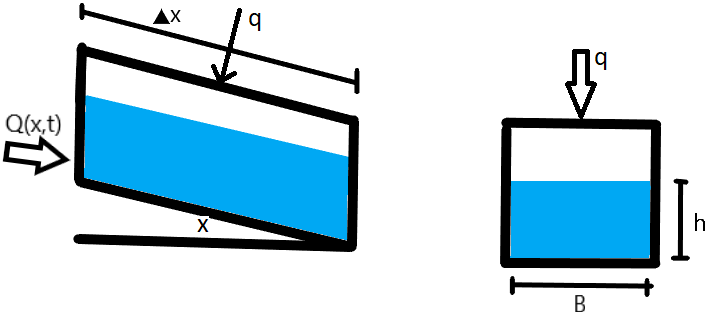
\includegraphics[width=0.45\textwidth]{report/modeling/pictures/firkant_kloak.png}
\caption{Flow in a channel with a flat bed and vertical sides where Q is flow into the channel, q is lateral flow into the channel and the cross section area is given by $\text{A} = \text{B} \cdot \text{h}$. \fxnote{Ny tegning}}
\label{fig:firkant_kloak}
\end{figure}

Flows, Q(x,t), q(x,t) and wetted cross section A(x,t) shown in figure \ref{fig:firkant_kloak} is dependent on time and position, but in the following a simpler notation is used for an easier outline. 

The flow into the control volume when considered from the center of the control volume is given as

\begin{equation}
	\left(Q - \frac{\partial Q}{\partial x}\cdot \frac{\Delta x}{2}\right) \cdot \Delta t + q \cdot \Delta x \cdot \Delta t
\label{flowin_saintbernard}
\end{equation}

Where q is the lateral inflow across the entire channel $\frac{m^2}{s}$ and Q is the flow in the channel $\frac{m^3}{s}$. Lateral inflow could for example come from adjoint sewer pipes or a gutter drain.
The discharge flow of the channel is given as

\begin{equation}
\left(Q + \frac{\partial Q}{ \partial x} \frac{\Delta x}{2} \right) \cdot \Delta t 
\label{flowout_saintbernard}
\end{equation}

and the change in stored fluid in the channel is given as

\begin{equation}
\begin{array}{l}
\frac{\partial}{\partial t} \left(\frac{\Delta x}{2} \cdot \left(A- \frac{\partial A}{\partial x} \frac{\Delta x}{2} +A + \frac{\partial A}{\partial x} \frac{\Delta x}{2}	\right) \right) \\
\Updownarrow \\
\frac{\partial A}{\partial t}\cdot \Delta t \cdot \Delta x	
\label{stored_saintbernard}
\end{array}
\end{equation}

As the flow into the channel is equal to the flow out plus the change in stored fluid in the channel, then due to the assumption of incompressible fluid and uniformity, \ref{flowin_saintbernard}, \ref{flowout_saintbernard} and \ref{stored_saintbernard} can be combined into equation \ref{saintbernard_masse}. 

\begin{equation}
\begin{array}{l}
	\left(Q - \frac{\partial Q}{\partial x}\cdot \frac{\Delta x}{2}\right) \cdot \Delta t + q \cdot \Delta x \cdot \Delta t - \left(Q + \frac{\partial Q}{ \partial x} \frac{\Delta x}{2} \right) \cdot \Delta t - \frac{\partial A}{\partial t}\cdot \Delta t 
	\cdot \Delta x = 0 \\ 
\Updownarrow \\
q \cdot \Delta x \cdot \Delta t -\frac{\partial A}{\partial t} \cdot \Delta t 
	\cdot \Delta x - \frac{\partial Q}{\partial x} \cdot \Delta x \cdot \Delta t  = 0 
\end{array}
\label{saintbernard_masse}
\end{equation}

Equation \ref{saintbernard_masse} can be reduced to the following by isolating and dividing with $\Delta x$ and $\Delta t$, on both sides, yielding the mass conservation part of the Saint-Venant equations.
\begin{equation}	
\frac{\partial A(x,t)}{\partial t} + \frac{\partial Q(x,t)}{\partial x}=q(x,t)
\label{saintbernard_mass_lateral}
\end{equation}

For channel flows without lateral input the mass conservation is given as:
\begin{equation}	
\frac{\partial A(x,t)}{\partial t} + \frac{\partial Q(x,t)}{\partial x}=0
\label{saintbernard_mass}
\end{equation}

Momentum of the control volume $\Omega$ shown in figure \ref{fig:kloakroer} \fxnote{figure mangler}can be found by utilizing Newtons second law which says that force is equal to mass times acceleration.
Basically this means that the momentum of the control volume can be found by integrating the sum of forces in the following differential equation.
\begin{equation}
	\frac{d \mathcal{M}(t)}{dt} = \sum_{i}F_i(t)
\end{equation} 
Where $\mathcal{M}$(t) is the momentum, given as mass times a velocity vector, of the control volume at time t and $\text{F}_i$(t) is the various external forces affecting the control volume.

The momentum given by the fluid particles at the cross section at each end of the control volume is given as
\begin{equation}
	\rho \cdot V \cdot Q
\end{equation}

where $\rho$ is density $\frac{kg}{m^3}$, v is velocity $\frac{m}{s}$ and Q is flow $\frac{m^3}{s}$.
The momentum given by the in- and output of fluid particles in the control volume, with the assumption that the density of the fluid and the velocity of it in the cross section of the control volume is constant, is given as
\begin{equation}
\begin{array}{l}
\rho \cdot v \cdot Q - \frac{\partial}{\partial x}(\rho \cdot v \cdot Q) \cdot \frac{\Delta x}{2} - \left(\rho \cdot v \cdot Q - \frac{\partial}{\partial x}(\rho \cdot v \cdot Q) \cdot \frac{\Delta x}{2} \right) \\
\Updownarrow \\
\rho \cdot \frac{Q}{A} \cdot Q - \frac{\partial}{\partial x}(\rho \cdot \frac{Q}{A}  \cdot Q) \cdot \frac{\Delta x}{2} - \left(\rho \cdot \frac{Q}{A}  \cdot Q - \frac{\partial}{\partial x}(\rho \cdot \frac{Q}{A}  \cdot Q) \cdot \frac{\Delta x}{2} \right)
\end{array}
\label{mass_flow_speed}
\end{equation}

The remaining to be found is the forces imposed by gravity, friction and the pressure.
The force applied by gravity is given as
\begin{equation}
F_g = sin(\theta)\cdot g \cdot \rho \cdot \Delta x \cdot A
\label{gravity_force} 
\end{equation}

where the slope of the pipe bed $\text{S}_\text{b} = tan(\theta) \approx sin(\theta)$ for small values of $\theta$ resulting in:
\begin{equation}
F_g = S_b \cdot g \cdot \rho \cdot \Delta x \cdot A 
\end{equation}
The friction force can be set up similarly as
\begin{equation}
F_f = S_f \cdot g \cdot \rho \cdot \Delta x \cdot A 
\label{friction_force} 
\end{equation}
where $S_f$ is a friction coefficient. This coefficient can be estimated by different formulas like Manning's or Darcy-Weishbach formula which is seen in equation \ref{Manning_formula} and \ref{darcy_weisbach_formula} respectively . 
\begin{equation}
	S_f = \frac{n^2 Q^2}{A^2R^{4/3}}= \frac{n^2 v^2}{R^{4/3}}
\label{Manning_formula}
\end{equation}
\begin{equation}
	S_f = \frac{f Q^2}{8gR A^2}= \frac{f v^2}{8gR}
\label{darcy_weisbach_formula}
\end{equation}

Where n is Manning's roughness factor, f is the Weisbach resistance coefficient and R is the hydraulic radius given as wetted area divided by the wetted perimeter \cite{stormwatercollectionsystems}.
The Weisbach resistance coefficient is found by the Colebrook-White formula seen in equation \ref{colebrook_white_formula}.
\begin{equation}
\frac{1}{\sqrt{f}} = -2\cdot log \left( \frac{k}{14.84 \cdot R}+ \frac{2.52}{4 Re \sqrt{f}} \right)
\label{colebrook_white_formula}
\end{equation}

Where f is the Darcy-Weisbach resistance coefficient, k is a pipe roughness coefficient and Re is the Reynolds number.

Last the pressure forces on the x component of the control volume to be found is marked as $P_1$ to $P_3$ in figure \ref{fig:forces_on_CV} 

\begin{figure}[H]
\centering
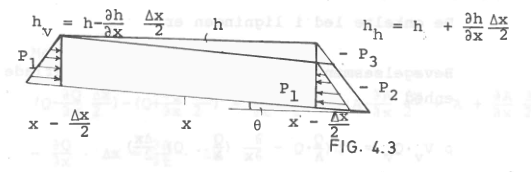
\includegraphics[width=0.75\textwidth]{report/modeling/pictures/palle_fig.png}
\caption{Forces acting on the control volume \fxnote{Ny tegning og sikkert også caption}}
\label{fig:forces_on_CV}
\end{figure}

The pressure forces acting on the control volume is given as:
\begin{equation}
	P_1 = \int_{0}^{h_l} \rho \cdot g (h_l - z)\cdot b(z)
\end{equation}
\begin{equation}
	P_2 = -\int_{0}^{h_r} \rho \cdot g (h_r - z)\cdot b(z)
\end{equation}
\begin{equation}
	P_3 = -\int_{h_l}^{h_r} \rho \cdot g (h_r - z)\cdot b(z)
\end{equation}
The total pressure force adds up to:
\begin{equation}
P_1 - P_1 -P_2 - P_3 = -\rho\cdot g \cdot \frac{\partial h}{\partial x} \cdot \Delta x \cdot A  
\label{pressure_force}
\end{equation}
Adding equation \ref{mass_flow_speed}, \ref{gravity_force}, \ref{friction_force} and \ref{pressure_force} an expression is given for the velocity of storing fluid in the control volume which is equal to:
\begin{equation}
\frac{\partial}{\partial t} (\rho \frac{Q}{A}A\cdot \Delta x)
\end{equation}
Entering the expressions of the conservation of momentum equation then the following is given:
\\
\begin{equation}
\begin{array}{l}
\rho \cdot \frac{Q}{A} \cdot Q - \frac{\partial}{\partial x}(\rho \cdot \frac{Q}{A}  \cdot Q) \cdot \frac{\Delta x}{2} - \left(\rho \cdot \frac{Q}{A}  \cdot Q - \frac{\partial}{\partial x}(\rho \cdot \frac{Q}{A}  \cdot Q) \cdot \frac{\Delta x}{2} \right)\\
-S_b \cdot g \cdot \rho \cdot \Delta x \cdot A -S_f \cdot g \cdot \rho \cdot \Delta x \cdot A  -\rho\cdot g \cdot \frac{\partial h}{\partial x} \cdot \Delta x \cdot A =\frac{\partial}{\partial t} (\rho \frac{Q}{A}A\cdot \Delta x)
\end{array}
\end{equation}
\\
Dividing with $\Delta x \rho g A$ and isolating then the definition of the equation is obtained.
\\
\begin{equation}
\frac{1}{gA} \frac{\partial Q}{\partial t} +\frac{1}{gA}\frac{\partial}{\partial x} \left( \frac{Q^2}{A} \right) + \frac{\partial h}{\partial x} + S_f - S_b = 0
\label{saintbernard_momentum}
\end{equation}
\\


%\begin{figure}[H]
%\centering
%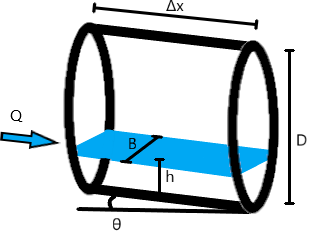
\includegraphics[width=0.45\textwidth]{report/modeling/pictures/kloakroer.png}
%\caption{Sewer pipe \fxnote{Ny tegning indsæt omega i control volumet}}
%\label{fig:kloakroer}
%\end{figure}


%\begin{equation}
%\frac{1}{gA} \frac{\partial Q}{\partial t} +\frac{1}{gA}\frac{\partial}{\partial x} \left( \frac{Q^2}{A} \right) + \frac{\partial h}{\partial x} + S_f - S_b = 0
%\label{saintbernard_momentum}
%\end{equation}

%\begin{equation}
%\frac{1}{gA} \frac{\partial Q}{\partial t} +\frac{1}{gA}\frac{\partial}{\partial x} \left( \frac{Q^2}{A} \right) + cos (\theta) \frac{\partial h}{\partial x} + S_f - S_b = 0
%\end{equation}



%\begin{equation}
%	\frac{\partial Q(x,t)}{\partial t} + \frac{\partial}{\partial x} \frac{ Q^2(x,t)}{A(x,t)}+ g \cdot A(x,t) (\frac{\partial h(x,t)}{\partial x} +S_f(x,t)-S_b(x)) = 0
%\label{saintbernard_momentum}
%\end{equation}




